% THIS IS ICT4S_PROC.TEX - VERSION 1.0 based on SIGPROC_SP.TEX (ACM SIG Proceedings Latex format)
% WORKS WITH V1 OF ICT4S_PROC_ARTICLE.CLS based on ACM_PROC_ARTICLE_SP.CLS V3.2SP
% August 2012
%
% It is an example file showing how to format the full paper for the ICT4S 2013 conference proceedings
%
% LaTeX2e document class file for Conference Proceedings submissions.
% ----------------------------------------------------------------------------------------------------------------
% ---------------------------------------------------------------------------------------------------------------
% It is an example which *does* use the .bib file (from which the .bbl file
% is produced).
%
% For tracking purposes - this is based on sigproc-sp V3.1SP - APRIL 2009


% NOTE ON THE DIFFERENCES:
% We have slightly tweaked the .cls and the .tex to allow a result similar to the 
% Word template provided for the ICT4S 2013.
% Authors:
% - below the title the authors are given as a centered list with footnote-like 
%   marks pointing to affiliations  (use \amarks{<number>} )
% - below the list of authors follows a list of addresses 
%     *each starting on a new line
%     *explaining one of the marks used in the list of authors
% - each address consists of the affiliation followed by the email addresses of the
%   authors belonging to the affiliation, an empty line before each affiliation
% - One email per author suffices
% 

\newcommand{\amark}[1]{\raisebox{5pt}{\small $#1$}}

\documentclass{ict4s_proc_article}
\usepackage{cite}
\usepackage{url}


\begin{document}

\title{Makahiki+WattDepot: An open source software stack for 
next generation energy research and education}

%
% You need the command \numberofauthors to handle the 'placement
% and alignment' of the authors beneath the title.
%
% Do not use the \alignauthor commands.

\numberofauthors{6} % necessary for working with the adapted style

\author{
% precede each author name, affiliation/snail-mail address and
% e-mail address. Additionally, tag each line of
% affiliation/address with \affaddr, and tag the
% e-mail address with \email.
%
 Philip M. Johnson, 
 Yongwen Xu,
 Robert S. Brewer,\\
 Carleton A. Moore,
 George E. Lee,
 Andrea Connell \\
 \\ % an empty line before each new affiliation
       \affaddr{Collaborative Software Development Laboratory, University of Hawaii at Manoa, Honolulu, HI 96822 USA}\\
\email{[johnson, yxu, rbrewer, cmoore, gelee, connell4]@hawaii.edu}\\
}

\date{19 August 2012}

% The editor remark on the first page at the bottom of the first column 
% is necessary!
\editorremark{
\hrule\par\rule[-0.65em]{0pt}{0em}\\
ICT4S 2013: Proceedings of the First International Conference on
Information and Communication Technologies for Sustainability, ETH Zurich, 
February 14-16, 2013. Edited by Lorenz M.~Hilty, Bernard Aebischer, G{\"o}ran Andersson and Wolfgang Lohmann.\\ \noindent http://e-collection.library.ethz.ch} %%W

\maketitle
\begin{abstract}
The accelerating world-wide growth in demand for energy has led to the conceptualization
of a ``smart grid'', where a variety of decentralized, intermittent, renewable energy
sources (for example, wind, solar, and wave) would provide most or all of the power
required by small-scale ``micro-grids'' servicing hundreds to thousands of consumers. Such
a smart grid will require consumers to transition from passive to active participation in
order to optimize the efficiency and effectiveness of the grid's electrical capabilities. 
This paper presents a software stack called comprised of two open source software systems,
Makahiki and WattDepot, which together are designed to engage consumers in energy issues
through a combination of education, real-time feedback, incentives, and game mechanics. We
detail the novel features of Makahiki and WattDepot, along with our initial experiences using
them to implement an energy challenge called the Kukui Cup.

\end{abstract}

%NO Categories 
%NO Terms

\keywords{smart grid, energy research, open source, game engine, energy repositories}

\chapter{Introduction}\label{chapter_introduction}
\textit{The central issue I address in the dissertation is a possibility of recurrent behaviors discovery from 
publicly available software process artifacts by leveraging data mining and knowledge discovery techniques. 
In particular I explored an approach of discovering of recurrent behaviors through the mining of time series that
are constructed by temporal ordering of measurements extracted from software process artifacts.
Further, I shall propose a novel technique for characteristic patterns discovery from time series and show its 
applicability to the problem at hands.}

\textit{The problem's background is provided in the Section \ref{section_background}. 
Section \ref{section_software_process_design} presents classical approaches for software process design and shows its limitations.
Section \ref{section_research_hypothesis} introduces the research hypothesis.
Section \ref{knowledge_discovery} provides a background into the problem of knowledge discovery 
from time-series.
Section \ref{section_trajectory_definition} connects two problems and provides definitions.
Section \ref{section_contributions} enumerates main contributions of the thesis, 
while section \ref{section_organization} explains the thesis organization.}

%
% >> section
%
\section{Background}\label{section_background}
Contemporary software projects concern with development of complex software systems and typically have 
a considerably long life-cycle - well over decade.
A project's development and maintenance activities are usually carried out by geographically 
distributed teams and individuals. The development pace, the experience, and the structure of the 
development team continuously change with project progression and as developers joining and leaving. 
When combined with schedule and requirements adjustments, these create numerous difficulties 
for developers, users, and stakeholders, ultimately affecting the project success \cite{citeulike:2207657}. 

This software development complexity phenomena was identified in 1968 as ``Software crisis'' 
\cite{naur_crisis_68}, and was addressed by bringing the research and the practice of software development 
(or as it was called ``programming'') under the umbrella of Engineering - in an effort to provide 
the control over the process of software development. 
Following the engineering paradigm, numerous methodologies and models of software design and development 
process, known as \textit{software processes}, were proposed \cite{citeulike:10002165}.

\begin{defn}\label{def_process}
A \textbf{\textit{Software Process}} defines a sequence of activities performed in order 
to design, develop, and maintain software systems.
\end{defn}
Examples of such activities include requirements collection and creation of UML diagrams, 
requirements testing, code development,  testing, etc. The intent behind a software process is 
to provide a control over software evolution by implementing a global strategy and by structuring
and coordinating human activities in order to achieve the goal - deliver a functional software system 
on time and under the budget. 

Since then, much research has been done on software processes resulting in a number
of software development models and paradigms. Some of these were widely accepted by practitioners 
and evolved into industrial standards for software development processes such as CMM, ISO, PSP, 
and others \cite{citeulike:5043104}. However, in spite of this effort, industrial software 
development remains error-prone and more than half of all 
commercial software development projects ending up failing or being very poorly executed 
(Rubinstein, ``Chaos Reports'', 2006) \cite{chaos2006}. Some of them are abandoned due to running 
over budget, some are delivered with such low quality, or so late, that they are useless, and some, 
when delivered, are never used because they do not fulfill requirements. 

Through the analyses of software project failures, it was acknowledged, that the engineering 
paradigm might not be the best way to provide a control over software development processes 
(\cite{citeulike:3729379} \cite{citeulike:5203446}) due to the fact that Software engineering 
is dealing with significantly different from other Engineering fields problems \cite{citeulike:2207657} .
The chief argument supporting this point of view is the drastic difference in the cost model:
while in Software Engineering there is almost no cost associated with materials and 
fabrication, these usually dominate cost in all other Engineering disciplines, but, 
ironically, Software Engineering is suffering from the costs and challenges associated with 
continuous re-design of the product and its design processes - the issue which is 
hardly seen at all in other Engineering areas. 
Further, it was found, that most of the engineering-like models are rigid, ``context-free'',
and rather prescriptive, i.e. they are universally defined independently of a particular 
organizational structure or a project specificities \cite{sacchi_2001}, and while they 
structure processes and provide the control, following them does not guarantee the success.
Yet another argument supporting alternative to engineering approaches is the increasing 
understanding and appreciation of a human role in software development processes over tools, 
technologies, and standards \cite{citeulike:6580825} \cite{citeulike:149387}
\cite{1605185} \cite{citeulike:113403} \cite{1605188} \cite{citeulike:12743107}. 

Along with Software Engineering, a number of alternative, flexible and user-oriented software processes 
emerged from academy, hobbyists, and practitioners addressing aforementioned issues \cite{citeulike:3729379}. 
Among others, the Free/Libre/Open-Source Software model (FLOSS) and the software craftsmanship  
approaches gained a significant credibility in community. 
While the former \textit{holistic} software process paradigm emphasizes loosely-organized 
collaboration, frequent releases, and effectively removes the boundary between developers 
and customers, the latter, human-centric approach, is built upon the roles of highly 
motivated skilled individuals \cite{citeulike:262020} \cite{citeulike:2759198}. 

Nevertheless, alternative processes were found to be plagued by the same complexity issues. 
As it was shown, most of FLOSS projects never reach a ``magic'' 1.0 version \cite{citeulike:12480029}. 
Among others, the great "infant mortality rate" of FLOSS projects was related to a burnout, 
inability to acquire a critical mass of users, loss of leading developer(s), and forking \cite{richter2007critique}. 
Software craftsmanship, from other hands, not only challenges developers with technological advances 
requiring continuous skills improvement, but creates significant cost and effort estimation difficulties for
stakeholders and project managers \cite{citeulike:11058784}. However, despite to these issues, 
the alternative processes proved that the disciplined manner of programming and the modularization  
of the software are capable of delivering large and reliable software systems, most notable Linux OS,
suggesting that community-driven processes as good as industrial engineering-like processes.

Currently, it is widely acknowledged, that there exists no single ``silver bullet'' process which 
can bring a software development project to success \cite{citeulike:1986013}. 
Processes are numerous, each has advantages and drawbacks, and each is accompanied with 
numerous application recommendations, success stories, and with failure experiences. Nevertheless,
the alarming rate of failing projects suggests that our understanding of software process ``mechanics''  
is limited and insufficient\cite{citeulike:12550665}. 
The enormous cost of the lost effort, measured in hundreds of billions of US dollars 
\cite{citeulike:2207657} \cite{citeulike:2207653} \cite{citeulike:2207655}, 
continues to provide motivation for further research on software processes. 

%
% >> section
%
\section{Software process design}\label{section_software_process_design}
Traditionally, approaches to software process design and improvement are divided into two distinct categories. 

The first category of software process design approaches consists of traditional to engineering 
\textit{top-down} prescriptive techniques through 
\textit{proposing a process based on specific patterns of software development}. 
For example, the Waterfall Model process proposes a sequential pattern in which developers first create a 
Requirements document, then create a Design, then create an Implementation, and finally develop Tests. 
The Test Driven Development process, from other hands, proposes an iterative behavioral pattern in which
the developer must first write a test case, then write the code to implement that test case, then re-factor the 
system for maximum clarity and minimal code duplication \cite{citeulike:6086365}. 

While the top-down approach follows the usual path of trials and errors, and seems to be an extension 
of natural to humans creative processes of invention and experimentation, 
the ``invention'' of an adequate to the task software process is far from trivial 
\cite{citeulike:5043104} \cite{citeulike:1986013}. Moreover, an evaluation cycle of an invented process
is usually very expensive and considerably long.
In addition, it was shown that the process inventors are often limited in their scope and tend to assume 
idealized versions of real processes, thus, often produce ``paper lions'' - process models which are 
likely to be disruptive and unacceptable for end users, at least in their proposed form 
\cite{citeulike:9758924}, which creates a large discrepancy between actions that supposed to be done for 
the novel process and what was actually performed by particular individual or the team.

The second category of software design approaches consists of \textit{bottom-up} techniques 
that focus on a \textit{performed process reconstruction through noticing of recurrent development 
events and behaviors} or as it also called \textit{process enactment}. 
Usually, the process reconstruction task is viewed as a two-levels problem where the first level 
consists of a patterns discovery (segmentation) while the second level consists of patterns recognition 
and their network analysis \cite{citeulike:2703162}.
One of the first works in this category was by Cook and Wolf, where they show a
possibility of automated extraction of a process model through the mining of recorded 
process event logs \cite{citeulike:328044} \cite{citeulike:5120757} \cite{citeulike:5128143}. 
Later work by Huo et al. shows that it is also possible to improve an existing process
through the event logs analysis \cite{citeulike:7691059} \cite{citeulike:7690766}. 

While the bottom-up approaches seem to be more systematic and potentially less complex than invention, 
they also affected by a number of issues. A chief among these is the observability issue - 
it is usually very difficult to conduct a full depth study on a live project due to the privacy concerns. 
Moreover, it is expensive to observe a process performed by a team for a whole life-cycle of a project. 
Yet another issue is the capacity of currently available process discovery techniques - 
typically these need to be supervised by experts and finely tuned in order to reconstruct 
distributed and concurrent processes. 

Nevertheless, despite to their differences, both techniques for software process design are 
producing process models that effectively are the series of actions that must be performed successively 
(sequentially and sometimes iteratively) in order to deliver a software. 
In order to produce the viable model, the ``process inventors'' put the best of their knowledge, experience,
creativity, and logical reasoning into the proposed sequence of steps, while ``process re-constructors 
strive to eliminate the noise and to converge to a concise process model that is supported by the 
majority of observations. 
This attention to synthesis of sequential steps, leaves other phenomenas, such as team's structure, work schedule, 
developer's discipline, their behaviors, and motivation behind. While this issue was recognized previously
and resulted in a number of studies which called for attention of human element in software production 
\cite{citeulike:149387} \cite{citeulike:113403} \cite{citeulike:205322} \cite{citeulike:12798652}, 
it is still largely ignored in industrial practices \cite{citeulike:12798659}, mostly due to the 
difficulties in benefit estimation \cite{citeulike:12798662} \cite{csdl2-12-11}.

%
% >> section
%
\section{Free/Libre Open Source processes}\label{floss_processes}
Along with growing amount of publicly available software, it became obvious, that self-organizing communities of 
mostly ``recreational'' software developers and active users are capable to successfully manage large code base, 
but to deliver software increasingly complex and surprisingly popular.
Many of large, ``global'' open source software development projects, such as Linux and its derivatives, 
Gnome, Apache HTTP Server, MySQL, and others, not only have comparable with industrial projects development team 
and code-base sizes, but the same average defect rate \cite{coverity2012}. 
These facts have attracted a considerable attention from industry and many organizations 
seek to emulate successful open source software processes in traditional ``closed source'' environment 
\cite{oss_virtual_organizations} \cite{oss_balance} \cite{oss_hp} \cite{oss_4industry}. 

\begin{figure}[ht!]
   \centering
   \includegraphics[width=140mm]{figures/Linus.Kernel.ps}
   \caption{A Torvald's response suggesting that practical reasons, the ``real-life'', should be always considered 
   over specifications.
   Excerpt from the Linux mailing list. \url{http://lkml.indiana.edu/hypermail/linux/kernel/0509.3/1441.html}}
   \label{fig:kernel}
\end{figure}

If we consider this as an assertion that open-source software processes are at least as good as engineering-like 
software process models, then, the freely available open-source process software artifacts potentially bear an 
incredible wealth of the information worth of studying. Moreover, the striking differences of open-source processes 
from a traditional software development could potentially reveal novel software processes and their aspects that 
were previously not accounted for. 
For example, consider that the most significant document in industrial software processes - a specification - 
is rarely considered at all in open source world. In FLOSS projects the software look and its functionality are 
rather viewed as open-end questions. Even in the Linux kernel development, which is probably one of the few strictly 
moderated FLOSS development processes, developers prise practical reasons over specifications 
\ref{fig:kernel}.

Yet another source of motivation for studying of public FLOSS software process artifacts comes from the fact that 
in order to facilitate the distributed FLOSS software development processes, the community is highly encouraging
developers to commit their changes rather often \cite{so-checkin} \cite{git-best-practices1}.
The frequent commits and the changes visibility practice is often cited as vital for health of software 
process as mentioned in some lengthy discussions: ``\textit{Don't Go Dark}'' \cite{checkin-dgd-2008}, 
``\textit{Check In Early, Check In Often}'' \cite{checkin-ch-2012}. Potentially, frequent commits create artifacts 
trails that provide finer resolution into project development and allow more thorough process recovery.

%
% >> section
%
\section{Public software repositories}\label{section_public_repositories}
Recently, the aforementioned situation changed, and the interest for process enactment and reconstruction, 
as well as attention to the human-specific components of software processes has been revived. 
This change is driven by the increase in public data that are made available by the proliferation of open 
source communities.

Currently, with accessible personal computers, friendly software development toolkits, and due to massification
of the use of the web as
a platform for collaborative work, small-scale commercial and recreational 
programming become very popular. 
Today, free code hosting sites such as SourceForge, GoggleCode, and GitHub host thousands of 
Free/Libre Open Source Software (FLOSS) projects.
These publicly offer numerous software artifacts such as design documents, source codes, bugs and issue records, and 
developers and users communications.
Further, Q\&A and social websites for developers such as StackOverflow, Biostars, TopCoder and others becoming 
increasingly popular among the software developers as places for exchanging experiences, learning new tricks, and 
improving skills, plus, they offer anonymized data back to the community.

The public availability of numerous software process artifacts effectively removes not only the high cost of observation, 
but most of the privacy concerns - the two issues that previously made any large-scale analysis of software projects 
unfeasible for most researchers.

Scientific community response on the availability of public artifacts was overwhelming, and a number of 
venues was established addressing the increased interest. 
Since 2004, the International Conference on Software Engineering (ICSE) hosts a Working Conference on 
Mining Software Repositories (MSR). The original call for papers stated MSR's purpose as 
\textit{``... to use the data stored in these software repositories to further understanding of software 
development practices ... [and enable repositories to be] used by researchers to gain empirically based 
understanding of software development, and by software practitioners to predict and plan various aspects 
of their project''} \cite{msr2004} \cite{citeulike:7853299}. 
Several other venues: International Conference on Predictive Models in Software Engineering \cite{promise12}, 
International Conference on Open Source Systems, the Workshop on Public Data about Software Development, 
and the International Workshop on Emerging Trends in FLOSS Research have also played
an important role in shaping and advancing this research domain.

Some of the published work addresses the software process discovery. Among others, most notable and 
relevant to my research is work by Jensen \& Scacchi. In their early work, they demonstrated, that 
information reflecting software processes can be gathered from public systems \cite{citeulike:12550640}. 
Later, in \cite{citeulike:5043664} and \cite{citeulike:5128808}, they show, that by manual mapping of 
collected process evidence to a pre-defined process meta-model it is possible to reconstruct some 
of the FLOSS processes. 
Another closely related to my research is work by Hindle et al. where they has shown that it is possible to 
discover software process evidence through partitioning \cite{citeulike:10377366}.

However, the research work based on mining of software process artifacts shows, that while public availability 
of artifacts is minimizing observability and privacy issues, the nature of these artifacts creates a number of 
challenges which I discuss in the chapter X, which limit the possible scope of the research and significantly 
elevate the complexity of the process discovery effectively rendering previously designed techniques inefficient.
Thus, the novel analysis and discovery techniques are needed to be developed for public software process artifacts 
analysis \cite{citeulike:7853299}.
% when ``\textit{... going beyond code and bugs...}'' 

%
% >> section
%
\section{Research hypothesis, scope of the dissertation}\label{section_research_hypothesis}
In previous sections, I have outlined the evidence of a limited performance of existing engineering-like 
software processes (Section \ref{section_background}),
as well the oversight of a variety of human factors that fall beyond a typical sequence of development 
actions by traditional approaches to software process design (Section \ref{section_software_process_design}).
Then, I have identified a few differences of FLOSS processes from traditional Software Engineering 
(Section \ref{floss_processes}), which can potentially shed light on human-driven aspects of software development.
Finally, I have pointed out a growing wealth of publicly available software process artifacts 
(Section \ref{section_public_repositories}) that is worth to explore for a better understanding not only 
FLOSS software processes, but their human factors. All this provided a motivation to my exploratory study, 
whose details I outline in this section.

In my work, I attempted to explore the possibility of discovery of a specific human-driven aspect in 
FLOSS software development that is a \textit{\textbf{behavior}}, which I define as the mannerism in which a 
developer, or a team, conduct their everyday work. 
In particular, I explore the possibility of discovery of \textit{recurrent behaviors}, i.e. behaviors supported 
by a numerous evidence, from software process artifacts. 

For example, if within an observation interval one developer frequently runs unit tests before committing 
changes into repository, while another usually commit changes without running the tests, the first developer's
habit of testing a code before the commit is a recurrent behavior that may reflect the developer's discipline,
or an unusual attention to some particular part of the code. 
Consider another example, if one of the developers usually commits code changes in mornings, while another 
developer late in the day, these two recurrent behaviors, might indicate a constraints that are put on the 
project, or the process, or on the developers themselves.
Obviously, latter behaviors should be possible to quantify by simple analysis of commit timestamps, while 
the former can be discovered by the analysis of co-occurring changes in the source code. 
Moreover, these and similar recurrent behaviors could be further associated with certain project's or process 
traits, such as pace, agility, size, complexity, code quality and others, which will not only extend our 
knowledge of human factors in software processes, but will lay a foundation for future research in software 
processes.

To begin with, I hypothesized, that \textbf{\textit{it is possible to discover recurrent behaviors from 
publicly available software process artifacts}}. 

Following the hypothesis, I have investigated a number of publicly available software repositories,
their artifacts, and a number of applicable data-mining techniques in a preliminary exploratory study 
\cite{csdl2-10-09}. However, similarly to other studies in the field, I have discovered, that while FLOSS 
process artifacts are numerous and readily accessible, their irregular, snapshot-like nature and the poor 
informational content significantly limit the applicability of known techniques for process mining.

In order to overcome this issue, I have casted the initial problem of event-based recurrent behaviors 
discovery into more generic problem of knowledge discovery from time series and approached it
by developing a novel technique for interpretable comparative analysis of time series that allows 
characteristic patterns discovery and ranking called SAX-VSM \cite{sax-vsm}. 

Further, I have developed a software artifacts analysis framework, called Software Trajectory Analysis, 
which aids in software artifacts collection, software process and product evolutionary metrics extraction, 
and their comparative analyses that enable discovery and ranking of characteristic patterns.


 in rank highlight is  transformation into  and by using I approached the problem of knowledge discovery 

developed a 
software process artifacts mining framework called Software Trajectory Analysis which is built upon 
a novel technique for comparative analysis of time series that allows characteristic patterns discovery 
and ranking.

This dissertation presents its results, as well as introduces a novel data mining technique designed to 
alleviate difficulties with interpretability of quantitative results obtained through mining of software
artifacts trails. 

%
% >> section
%
\section{Knowledge discovery from time series}\label{section_knowledge_discovery}
In data mining, time series are used as a proxy representing a vast variety of real-life phenomena 
in wide range of fields including, but not limited to physics, medicine, meteorology, 
music, motion capture, image recognition, signal processing, and text mining. 
While time series usually directly represent observed phenomenas by capturing their measurable evolution in time, 
the pseudo time series often used for representation of various high-dimensional data 
by combining data points into ordered sequences. 
For example in spectrography data values are ordered by component wavelengths \cite{citeulike:12550833};
in shape analysis the order is the clockwise walk direction starting from a
specific point in the outline \cite{citeulike:12550835}, in image classification the numbers of pixels
are sorted by color component values \cite{citeulike:2900542}.

Many important problems of knowledge discovery from time series reduce to the core task of finding 
characteristic, likely to be repeated, sub-sequences in a longer time series. 
In the early work these were called as 
\textit{frequent patterns} \cite{citeulike:5159615}, 
\textit{approximate periodic patterns} \cite{citeulike:1959582},
\textit{primitive shapes} \cite{citeulike:5898869}, 
\textit{class prototypes} \cite{citeulike:4406444}, 
or \textit{understandable patterns} \cite{citeulike:3978076}. 
Later, similarly to Bioinformatics, these were unified under the term \textit{motif} \cite{citeulike:3977965}.
Once found, motifs can be used for a hypothesis generation by finding their associations with known,
or unknown phenomenas \cite{citeulike:3977965}. 

The recent advances in semi-supervised and unsupervised finding of such characteristic sub-sequences, 
in particular work based on \textit{shapelets} \cite{citeulike:7344347} \cite{citeulike:11957982}
\cite{citeulike:12552293} and \textit{bag of patterns} \cite{citeulike:10525778}, show a great potential 
of application of time series data-mining techniques to a wide variety of high-dimensional data.

Unfortunately, both techniques provide a limited insight into the data and suffer from performance issues. 
While exact shapelet techniques allow discovery of class-characteristic patterns and facilitate classification,
algorithm is almost quadratic and provides limited insight into class specificities. 
The bag of patterns algorithm, while performs in a linear time, requires a previous knowledge for input parameters 
selection and does not offer class generalization.

In order to overcome this limitations, in this thesis I propose a novel approach for time-series classification and 
knowledge discovery that is called SAX-VSM and is based on symbolic approximation of time series and vector space model. 
As I shall show, SAX-VSM is capable to discover and to rank characteristic subsequences representing time series classes. 
The proposed algorithm not only facilitates classification, but provides insights into the both: classification results 
and time series classes specificities. As I shall show, by facilitating the class' characteristics patterns ranking,
SAX-VSM enables the discovery of recurrent behaviors and their heat-map like visualization. 

\section{Software trajectory analysis}\label{section_trajectory_definition}
Previously, Johnson et al. defined \textit{software metrics telemetry streams} \cite{citeulike:12550871}, 
(what they re?) and showed, that it is possible to improve software development process by using the 
knowledge extracted by experts through visual analysis of these streams.
 
Similarly to software metrics telemetry streams, I abstract software process artifact by collecting their 
metrics and arrange these measurements by artifact creation time into high-dimensional vectors. 
These non-equidistant, often sparse and uneven in length time series 
I call ``\textbf{software trajectories}''. Similarly to approximate trajectories of objects in 
a physical space, or reduced in complexity sequence of states of a dynamic system (Poincare' maps), 
the \textit{software trajectory is a curve that describes a software project progression in a space 
of a chosen metrics}.

Through an exploratory study, I have discovered, that by the comparative analysis of software trajectories 
with SAX-VSM it is possible to discover and to interpret recurrent behaviors. This workflow that 
consists of software artifacts collection, their metrics extraction, and comparative analyses I call 
\textit{\textbf{Software Trajectory Analysis}} (STA). 

In this thesis, through three case studies, I will show, that Software Trajectory Analysis is capable 
of discovering of a various characteristic patterns which ca be associated with recurrent behaviors.

\section{Contributions}\label{section_contributions}
Main contributions of my work can be summarized as follows: 
\begin{itemize}
\item I propose a novel, generic algorithm for interpretable time series classification: SAX-VSM. 
While the classification performance of this algorithm is at the level of current state of the art, 
it offers an outstanding feature - discovery, generalization, and ranking of class-characteristic features. 
This, in turn, enables knowledge discovery by offering much clearer insight into classification results than any of 
competing techniques.
In addition, SAX-VSM is very fast in classification and has a small memory footprint. 
Overall, I expect this algorithm to play an important role in future because of the growing ubiquity of time series and 
a growing interest in behaviors.
\item Powered by SAX-VSM, I design a Software Trajectory Analysis (STA) framework, and through case-studies 
show its capacity for recurrent behaviors discovery from publicly available software process
artifacts. While case studies are obviously limited, I argue that STA is a useful knowledge discovery tool applicable for a 
variety of software process artifacts and metrics. 
\item Finally, I provide SAX-VSM and STA implementations to community.
\end{itemize}

\section{Dissertation Outline}\label{section_organization}
The rest of this dissertation is organized as follows. Chapter \ref{chapter_background_work} discusses the history 
of Software Engineering, previous work in software process discovery, mining of software repositories, and current 
state of the art in time series mining. Chapter \ref{chapter_sax_vsm} proposes an algorithm for interpretable 
time series classification. Chapter \ref{chapter_sta} discusses the design of STA framework and presents case studies.
Chapter \ref{chapter_conclusions} concludes and discusses several directions for future study.

\section{WattDepot}

Software for energy collection, storage, and analysis tends to come in two flavors that support two ends of the scalability spectrum.  At one end are utility-scale SCADA systems and protocols which are intended to manage macro-grid data \cite{SmartEnergy2.0, OSHAN, OpenPDC}.  At the other end are ``personal scale'' systems such as those provided by energy meter or solar panel manufacturers which are intended to manage information about single households \cite{TED, EMS100}.  We designed WattDepot to support a middle ground that we refer to as ``enterprise-level'' energy management, in which data concerning energy production and consumption of hundreds to thousands of households can be usefully managed~\cite{csdl2-10-05}. Figure \ref{fig:wattdepot} illustrates the architecture of the system, where WattDepot sensors send data from meters attached to energy devices to a server, which can then be queried by clients to provide visualizations and analyses.

\begin{figure}
\begin{center}
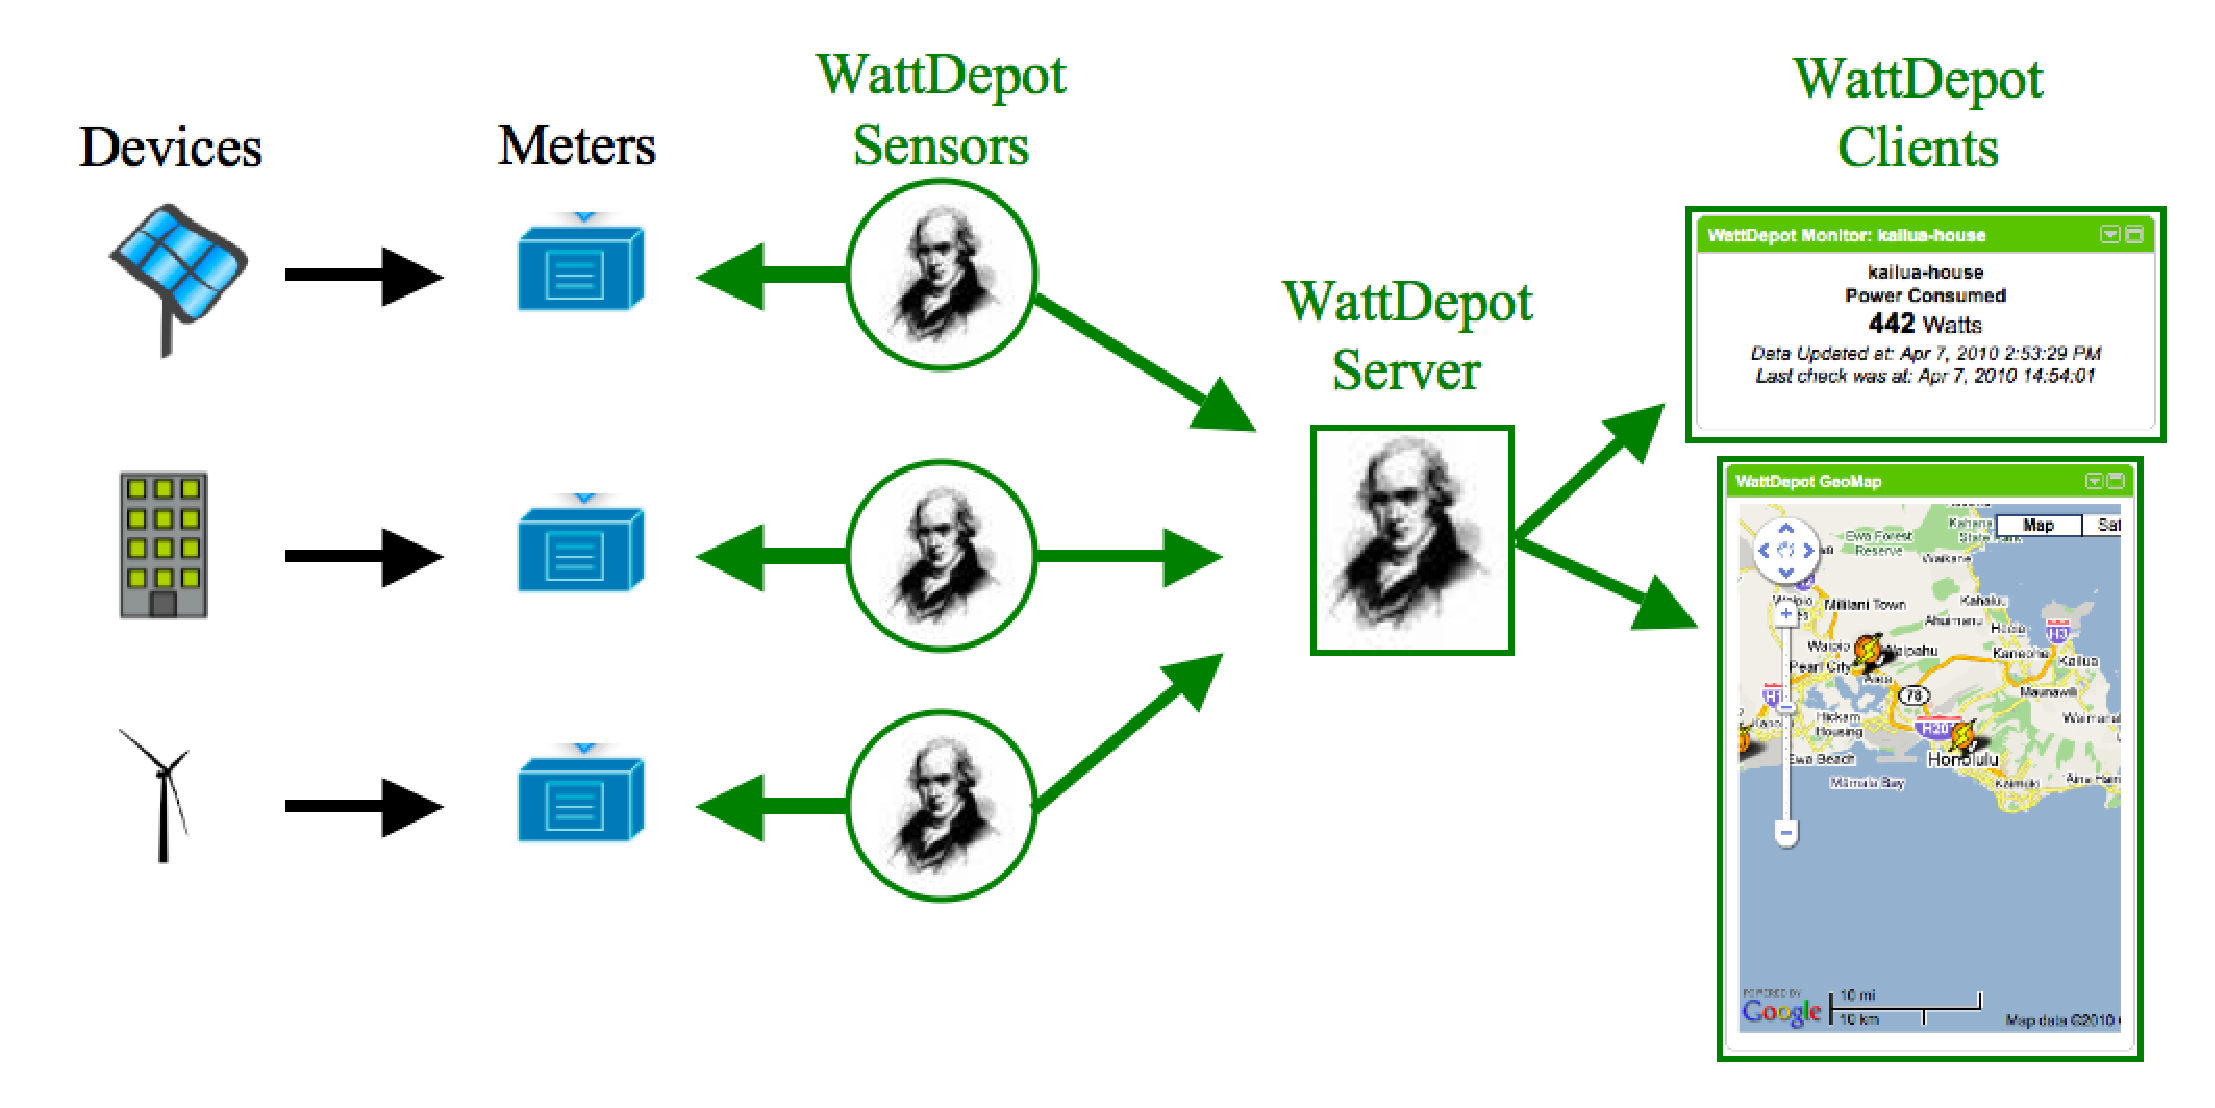
\epsfig{file=wattdepot-architecture, width=3in}
\end{center}
\caption{Architecture of WattDepot}
\label{fig:wattdepot}
\end{figure}

Our use of WattDepot has led to a novel set of capabilities to support this middle ground.

\subsection{Meter Agnostic}

Unlike personal-scale systems that are typically tied to a particular manufacturer's product, WattDepot is agnostic about the kinds of meters used to monitor energy production and consumption data, and whether the data is personal-scale or utility-scale. It provides a REST protocol for data transmission that can be used to implement clients for a wide variety of devices; the major constraint is that these devices need to have network access. WattDepot clients can be written in any language that supports the HTTP protocol. We provide a high-level client libraries for Java and JavaScript.

Due to the architectural decoupling of data collection from the rest of the system, WattDepot can be effectively used for simulation and what-if scenario development. This flexibility makes it appropriate as a kind of technological ``scaffolding'' for smart grid applications, where WattDepot can provide clients with simulated production and consumption data early in development, with the simulated data transitioning to live data as these sources go online later in development.

\subsection{Source Aggregation}

WattDepot can represent aggregations of power sou\-rces. For example, a building might have multiple meters monitoring energy consumption, one per floor. WattDepot can represent the power consumed by individual floors, as well as an aggregate source representing the building as a whole. Aggregations can be nested, so that floors can be aggregated into buildings, buildings into neighborhoods, and neighborhoods into cities. It is quite common for level of abstraction desired by client developers and end users (such as a floor of a building) to actually consist of multiple meters. By providing this aggregation of sources at the server level, client development becomes easier.

\subsection{Data Interpolation}

WattDepot automatically performs data interpolation when necessary. For example, a meter might provide a snapshot of energy usage once per hour for a given device. Clients can request the power consumed by this device at any time instant, and WattDepot will automatically provide interpolation when the requested time does not match a time for which actual sensor data is available. This is essential for the common case where meters do not have perfectly synchronized clocks and are not polled simultaneously, and when making use of the source aggregations discussed in the previous section.

\subsection{Flexible Data Storage}

WattDepot is architecturally decoupled from the underlying data storage technology. This supports experimentation with both traditional relational as well as NoSQL technologies, and facilitates scalability. Currently, WattDepot implements support for Derby, PostgreSQL, and BerkeleyDB storage systems. Administrators looking for simplicity may opt for the embedded Derby database, while those looking to integrate with existing database infrastructure might decide to use PostgreSQL for data storage.

WattDepot also implements support for ``ephemeral'' data. In some application scenarios, it is useful to send energy data to the WattDepot server quite frequently (i.e. every few seconds) so that clients can monitor current energy consumption with low latency. However, that rate of data sampling is not necessary for historical analyses, which may only require energy data sampling at the rate of every few minutes. WattDepot supports this situation through ephemeral data, which creates an in-memory window during which all recently received energy data is available for retrieval, but stored in the repository only at a much lower sampling rate.

\subsection{WattDepot in the Cloud}

In addition to installation on a local server, WattDepot has been designed to support cloud hosting, sometimes referred to as Platform-as-a-Service (PaaS). In particular, WattDepot can be deployed on the Heroku\footnote{http://www.heroku.com} cloud-based hosting service. The Heroku PaaS solution allows users to deploy the system and start collecting data without the requirement of server hardware, and Heroku offers flexible capacity depending on the expected workload.

\subsection{Beyond WattDepot}

While WattDepot provides the software infrastructure to collect, store, and analyze energy data, ensuring that the data is collected reliably and accurately reflects reality requires additional effort. As an example, we will examine the steps required to collect data on electricity use in a building. First, the administrator should work with manager of the building to understand the electrical infrastructure: how is power distributed in the building, and how does the distribution relate to the goals to be accomplished through measurement? If electricity is to be monitored at the per-floor level, do the distribution panels match that segmentation?

If the building does not have meters already installed, the administrator will need to select a meter vendor and acquire the meters. The meters will typically need to be installed by licensed electricians. The administrator will need to verify that the installation was performed correctly by checking whether the received data agrees with the expected amount of usage. To allow WattDepot to collect data, reliable network connectivity must be provided for the meters. The meters will also need to be configured to support remote data collection.

If the building already has meters installed, the administrator will need to confirm that the meters are configured correctly and that the data they produce  is sane. When working with existing meter infrastructure, the WattDepot administrator may not have administrative access to the meters, so any configuration changes required may need to be requested from the meter administrator.

Once data collection has been established, the WattDepot administrator will need to establish monitoring of the meters and WattDepot infrastructure so that hardware or software faults can be detected and corrected before they lead to excessive loss of data. By understanding these issues, administrators can ensure that systems built on top of WattDepot receive accurate energy data at appropriate levels of abstraction.


\section{Makahiki}
The feature set of WattDepot creates attractive infrastructure for management of energy data, but research suggests that effective participation of consumers in a next generation smart grid requires more than simple feedback to consumers about their consumption, particularly given the passive nature of their involvement for the past 100 years~\cite{Froehlich2010-BECC, Houde2013-powermeter, Pierce2012-BEM}.

The second component of our open source software stack, Makahiki, represents research intended to create synergy between the need to create knowledge and engagement regarding energy and the ability of so-called ``serious game'' techniques and energy feedback to create participation and engagement \cite{Deterding2011mt,darby-review-2006,Faruqui09,petersen-dorm-energy-reduction}. In Makahiki, online game mechanics are employed with the goal of affecting real-world energy behaviors~\cite{csdl2-10-07}.  The ultimate goal is to not just affect energy behaviors during the course of the game, but to produce long lasting, sustained change in energy behaviors and outlooks by participants. Figure \ref{fig:makahiki-architecture} illustrates the architecture of Makahiki.

\begin{figure}
\begin{center}
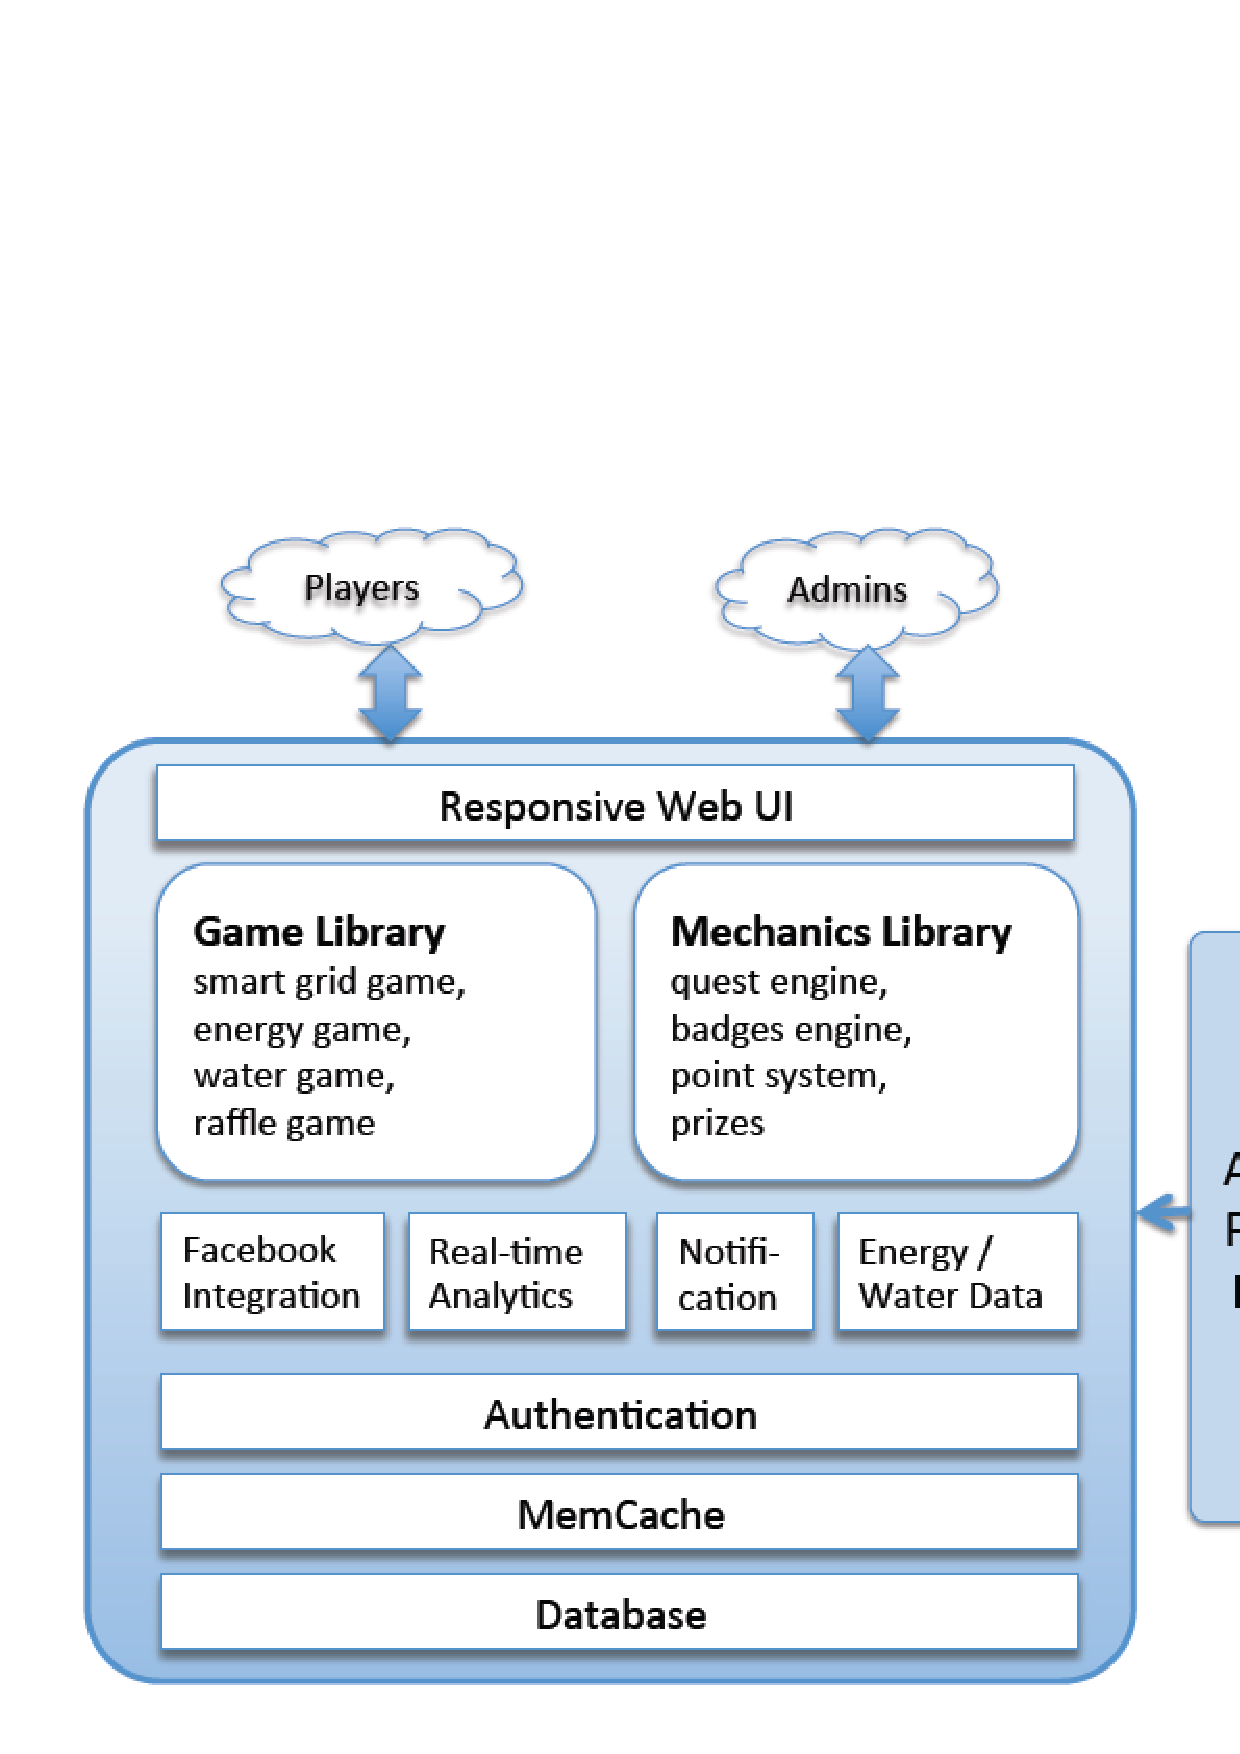
\epsfig{file=makahiki-system-architecture, width=3in}
\end{center}
\caption{Architecture of Makahiki}
\label{fig:makahiki-architecture}
\end{figure}

Makahiki consists of a configurable game engine that can be customized to the needs of different organizations.  It includes a library of pre-built game ``widgets'' that implement a variety of game mechanics.  Using the widgets, an organization can create a custom energy challenge in which players can compete individually and/or in teams to earn the most points by reducing their energy consumption as well as by learning about energy concepts in general.  The next sections present some of the most important widgets in Makahiki.

%\bigskip
\subsection{Smart Grid Game}

The Smart Grid Game widget shown in Figure \ref{fig:SmartGrid}, is the primary place players go to learn about energy issues and earn points. Actions are organized into a grid of squares (hence the name ``Smart Grid'') and organized by category columns. The game supports levels so that a large number of actions can be presented in a sequence of smaller grids. Each grid contains four different types of actions: activities, commitments, events, and excursions.

\begin{figure}[th]
  \center
  \includegraphics[width=0.95\columnwidth]{smart-grid.eps}
  \caption{\em Smart Grid Game widget}
  \label{fig:SmartGrid}
\end{figure}

{\em Activities} are the most basic actions available in the Smart Grid. In order to get points for an activity, a player will have to provide a response to the administrators. These responses can be a short textual answer or an uploaded picture. Administrators access a special section of the web application to approve or deny submissions. If a submission is approved, the player will receive the points for their submission, as well as a website notification about the approval. If the submission is rejected, the player will be sent an email notification informing them that their submission was not approved, and a textual description by the administrator of why it was rejected. The player can change and resubmit their response and still earn the full point value for that activity.

{\em Commitments} are pledges that the player will do something related to energy or sustainability for a period of five days. Examples include: reducing shower time, taking the stairs, and turning off the lights when leaving a room. Although these commitments are not verifiable, they are public and visible to other players in the same team and worth fewer points than activities. Furthermore, a player can only have up to five active commitments at any given time. After the five days period is up, the player can then declare that they completed the commitment and immediately earn their points. They can then sign up for another commitment, including the one they just completed.

{\em Events and excursions} are tied to real world activities. Events are held locally while excursions require transportation. Seating is limited, so players are asked to sign up for events or excursions they wish to attend. Players that do so are provided with a 2 point signup bonus. Players can also set up a reminder that is sent to their email and/or their mobile phone before the event takes place. At the event, an administrator will hand out attendance codes printed on slips of paper that can be entered on the website. These attendance codes are generated by Makahiki and can only be used once. To discourage players from signing up and not attending, a 2 point penalty is applied to players who do not submit an attendance code. If the player submits an attendance code for the event after receiving this penalty, the penalty is reversed.

Not all of the actions and levels in the Smart Grid Game are necessarily available at
the start of the game. We provide a set of predicates that can be used to determine if an action or level is locked or unlocked for a player. These predicates include: completed a certain number of actions within a category, completed all actions within a category, completed a certain action, and unlocked after a certain date (time-based unlocking).

These predicates are implemented using a limited subset of Python and can
be changed within the administrative interface. Challenge designers can use
logical operators to combine any of these functions in order to organize
the players' path through the Smart Grid Game.

\subsection{Power Meter}

A fundamental requirement for enabling more active participation by consumers in the smart grid is feedback regarding their energy usage.  One of the most simple mechanisms provided by Makahiki for this purpose is the Power Meter widget, illustrated in Figure \ref{fig:PowerMeter}.

\begin{figure}[th]
  \center
  \includegraphics[width=0.95\columnwidth]{power-meter.eps}
  \caption{\em Power Meter widget}
  \label{fig:PowerMeter}
\end{figure}

The Power Meter widget provides basic feedback on energy consumption via a display of the team's power consumption, updated every few seconds.  The visualization can normalized using baseline values so that when the needle is pointing straight up, the power consumption is the average for that team during that specific hour of that specific day of the week.  Thus, if the needle leans left toward the green side, the team's power consumption at that moment in time is below average, while if the needle leans right toward the red side, the team's power consumption at that moment in time is above average.  

The Power Meter widget obtains its values by querying the WattDepot system for the latest power data consumed by the associated team.  The use of WattDepot, rather than directly querying the meter(s), simplifies the widget design significantly.  First, the physical meters can vary significantly in the protocol implemented to obtain current power consumption.   These protocol variations are handled by the WattDepot sensors, so this widget can simply query the WattDepot server using a single HTTP request that is independent of the physical meter characteristics.  Second, the power consumed by a team might be measured by one or multiple meters.  Again, the WattDepot source aggregation capability means that this physical difference can be abstracted away by WattDepot, enabling the widget to obtain the aggregate power for the team through a single HTTP request.

The Power Meter widget is a useful, though simple mechanism for energy feedback that uses the WattDepot+Makahiki stack.   The next section presents a more sophisticated mechanism called the Daily Energy Goal Game.

\subsection{Daily Energy Goal Game}

The Daily Energy Goal Game widget provides a way for players to earn points by reducing their current energy consumption from a baseline. This baseline can be calculated using historical data or dynamically throughout the competition. Both the baseline data and the current consumption is typically provided by API calls from Makahiki to an underlying WattDepot server.
Figure \ref{fig:DailyEnergyGoal} illustrates this widget.

\begin{figure}[th]
  \center
  \includegraphics[width=0.95\columnwidth]{daily-energy-goal-game.eps}
  \caption{\em Daily Energy Goal Game widget}
  \label{fig:DailyEnergyGoal}
\end{figure}

The goal for each team is typically a percent reduction from their baseline usage. When a player goes to the energy page of Makahiki, they can view their team's current progress toward their daily energy goal. Near the end of the day, Makahiki checks the energy data from Wattdepot to see if a floor reached their goal. If the floor did reach their goal, each member of the floor that is participating in the game receives points. The energy goal game provides a link between the energy conservation competition and the point competition.

The Daily Energy Goal display shows both their current progress and their goal so far. We have noticed that our participants use more energy at night rather than during the day. Thus, it is easy to be under their actual energy goal for most of the day and then jump over the goal at the very end. Displaying their progress toward the goal so far provides a pace for players to follow.

\subsection{Raffle Game}

The Raffle Game widget provides a way to incentivize participation from all individuals, even those who are not in the running for a top prize. For every 25 points a player earns, they receive one virtual raffle ticket. Players can dynamically allocate their tickets to any raffle prizes they are interested in at any time, up to the end of the raffle. Figure \ref{fig:RaffleGame} shows an example of the Raffle Game.


\begin{figure}[th]
  \center
  \includegraphics[width=0.95\columnwidth]{raffle-small.eps}
  \caption{\em Raffle Game widget}
  \label{fig:RaffleGame}
\end{figure}

Each round of the competition has its own set of raffle prizes and any unused raffle tickets carry over to the next round. Raffle tickets are independent from a player's score, and allocating a raffle ticket does not affect their rank. The system will randomly pick the raffle winners at the end of each round.

\subsection{Social and Referral Bonuses}

The Social and Referral Bonus are the game mechanics that help encourage participation by providing additional points to players who participate in activities with other players and facilitate the entry of new players into the game.

The social bonus is an configurable option when an action is created in the Smart Grid Game. Players receive extra points if they perform the action with another player. Examples of actions with a social bonus include attending an event, recording a song related to energy, or measuring a shower water flow rate. When a player submits a response for an action with a social bonus, the player can provide the email address of the person who jointly completed the action. Once the other player completes the action, the social bonus is awarded. Social bonuses are not bi-directional; if the second player doesn't provide the first player's email address, only the first player will get the social bonus.

Players are led through a setup process when logging into Makahiki for the first time. One of the steps in this process is the referral bonus. If a player was referred by another player in the system, they can use this step to input their email address. Once the new player earns a certain number of points in the competition, both players are awarded a referral bonus of a configurable number of points. Typically, going through the setup process gives you 25 points, so setting a point threshold of 30 points encourages the new player to at least complete one additional action in order to get the referral bonus.

\subsection{Quest Engine}

One challenge we faced when designing Makahiki was providing adequate help to the player. The game needed to be intuitive, even if a new player coming to Makahiki is not familiar with an energy competition. Unlike many web applications, such as email, The Makahiki players generally do not know in advance what specific actions they wish to accomplish. In an effort to provide a player with guidance through Makahiki after the setup process, we implements the Quest Engine. Quests are used to guide a player through the various workflows of the site, such as completing an action, signing up for an event, or allocating a raffle ticket. These quests can be created using the administrative interface. Quests use a set of predicates to determine unlock and completion conditions. These predicates include: participating in a certain action or type of actions, completing a certain action or type of actions, having a certain number of points, completing a certain number of actions in a category or of a given type, being awarded a badge, and adding a picture to their profile.

\subsection{Game Analytics}

Makahiki is designed to support energy challenges involving hundreds or thousands of users lasting weeks or months.  In these circumstances, effective use of the technology requires the ability to understand the state of the game, such as: Who is using it? What are they doing? What is the player response to activities, commitments, excursions, and events?   Such state information is important for planning purposes, such as assessing the transportation needs for an upcoming excursion by seeing how many players signed up.   It can also be used for making in-game changes to game design, such as changing the point values associated with activities to encourage or discourage participation.  It can also help identify breakdowns in game play, such as significant numbers of unallocated raffle tickets indicating that users do not understand the nature of that game mechanic.  

To address these needs and others, Makahiki includes a variety of widgets that work together to provide high level overview of game play state to the administrators of a challenge. Figure \ref{fig:status} shows an example of two game analytic widgets.

\begin{figure}[t!]
  \center
  \includegraphics[width=0.95\columnwidth]{status.eps}
  \caption{Game analytic widgets: User Stats and Energy Goal Status}
  \label{fig:status}
\end{figure}

The top widget, User Stats, shows trends in the total number of players, the total number of new users, and the total number of players visiting the site each day.  The bottom widget provides information on the ability of teams to achieve their daily energy goal each day and over time.  

We have now introduced the primary components of our software stack, WattDepot and Makahiki.  The next section presents our experiences and lessons learned so far. 


\newpage
\section{Experiences}

To better understand the strengths and weaknesses of the Makahiki+WattDepot software stack, we have been designing and implementing an ``Energy Challenge'' called the Kukui Cup.  Development of the Kukui Cup challenge began in 2009, and the first Kukui Cup challenge was held in 2011 for over 1,000 first year students living in the residence halls at the University of Hawaii (UH) in Fall, 2011.  In Fall 2012, the second Kukui Cup challenge was held at the University of Hawaii using Makahiki+WattDepot.  In addition, Hawaii Pacific University (HPU) held a Kukui Cup challenge using Makahiki+WattDepot. Finally, an international organization called the East-West Center (EWC) held a Kukui Cup challenge using just Makahiki (their energy data was manually gathered by reading meters and entering the data by hand, so WattDepot was not needed for their challenge).    

The successful creation of four challenges by three different organizations over two years provides evidence that the software stack can be tailored to the differing needs of separate organizations.  First, UH uses meters by Electro-Industries Inc., while HPU uses meters by EGauge Inc., and EWC collected their energy data by hand. Second, while UH and HPU challenges involved only energy consumption data, the EWC challenge involved both energy and water consumption data.  Third, the IT infrastructure at UH and HPU provided authentication services using CAS and LDAP, while EWC used the built-in Django authentication. Fourth, the user interface was customized to ``brand'' each challenge with the logo and other thematic elements of the sponsoring organization. 

On the other hand, it should be recognized that these organizations are in other ways quite similar: they are all institutions of post-secondary education, and they are all based in Hawaii.  These organizational similarities are mostly due to the desire by the 2012 challenges to reuse a significant amount of the content developed in 2011, which was oriented toward the Hawaii-based, college aged demographic. For 2013 and beyond, we hope to expand our experiences with the software stack  ``downward'' into primary and secondary schools, and well as ``outward'' into residences and businesses. 

User response to the 2011 UH Kukui Cup challenge was positive, and provided evidence regarding the software stack's usability, functionality, and performance characteristics.   Over 400 students participated, for an adoption rate of approximately 40\%.  In a user survey conducted near the end of the challenge, over 90\% of users said they would participate in the challenge again if offered an opportunity.  60\%  said ``ease of use'' was the thing they liked best about the website.  40\% responded ``Nothing'' when asked what was confusing about the website, and 32\% responded ``Nothing'' when asked what they would change about the website.  The survey did yield insights into what could be improved, including the ability to introduce new games at points during the challenge, to provide better access to other player data, and simplify navigation.  There was virtually no downtime during the 2011 challenge, and only one significant bug in the system (affecting scoring) was discovered during the challenge, which was fixed within a day of its discovery.  Finally, a pre- and post-challenge survey questionnaire yielded statistically significant evidence that participants in the challenge learned more about energy concepts than those not participating, demonstrating that the approach can serve to improve consumer knowledge of energy as needed for active engagement with the Smart Grid.

The 2012 challenges are ongoing as of the time of writing, so the following results must be viewed as preliminary, but our current experience is similarly positive to 2011.  The UH challenge participation rate so far appears to be slightly lower than last year, at about 33\%, though the HPU challenge participation rate so far is higher (approximately 50\%), and the EWC participation rate is much lower (around 6\%). None of the challenge instnaces have experienced significant downtime, and so far only 1 significant bug (affecting scoring) has been reported (and has again been fixed within a day).  Load testing of the software stack just prior to the 2012 challenge indicates a hypothetical throughput of around 200 concurrent users with acceptable page loading times, though we have not experienced that level of load in the current challenges. 

Our experiences over the past two years has provided many lessons learned, and some of the most important regarding the Makahiki+WattDepot software stack are:

{\em Cloud-based hosting simplifies installation.}  During 2012, we have gained experience with both cloud-based hosting as well as local installation for the Makahiki+WattDepot software stack.  We have found that cloud-based hosting significantly simplifies the installation process and avoids certain types of installation-related bugs from occurring, particularly when system administrators are not familiar with the stack components that Makahiki+WattDepot depend upon (Django, Java, Python, git, etc.)  On the other hand, cloud-based hosting incurs costs (in our experience, between \$50-\$100/month for these challenges) and may incur constraints (for example, the Heroku hosting platform currently has minimal support for LDAP authentication).  The Makahiki Manual \cite{MakahikiManual} provides instructions for both cloud-based and local installation, providing some idea of the differences between the two approaches.  The lesson learned is to use cloud-based hosting when possible, or allow plenty of time for administrators to work through the software stack installation issues. Makahiki+WattDepot is not yet a ``plug-and-play'' system.

{\em Challenge design and administration is time consuming.} Despite the freely providing the Makahiki+WattDepot software stack to HPU and EWC, along with content developed specifically for college-age residents of Hawaii, the administrators still expressed surprise at the how time consuming it was to design and administrate the running of their respective challenges.  This appears to be due to the fact that the software stack enables a variety of game mechanics (such as the Smart Grid Game, Raffle Game, Badges, and point-based Prizes) not present in more simplistic energy challenges.  For example, the Smart Grid Game requires configuration of the widget including what activities to include and when/where they appear in the game.  The Raffle Game and point-based awards requires the collection of appropriate prizes. While we provided a library of almost 100 activities from 2011, all of the 2012 challenges required the definition of at least a few new events.  Thus, although the result is a more sophisticated experience for the participants, the up front design and overhead during execution was generally surprising to the administrators. The Kukui Cup Challenge Planning Guide \cite{KukuiCupChallengePlanningGuide} provides more details on this process.  The lesson learned is to make sure that potential organizational sponsors understand that the use of this software technology is not intended to make it more simple for them to run an energy challenge, but rather to enable them to create a more sophisticated energy challenge than would otherwise be possible.

{\em Scalability cuts across both design and implementation.}  So far, the use of the Makahiki+WattDepot software stack has been limited to relatively small user communities of 1,000 participants or less.  We believe that the system and approach would scale relatively well to some small number of multiples of that number, say to a maximum of 10,000 challenge participants.  On the other hand, there are both design and implementation challenges in scaling the software stack to communities of significantly larger than 10,000 participants.

On the design side, Makahiki currently requires administrators to approve each submission by a participant in order for that participant to receive points.   In the UH challenges, that results in administrative approval of around 4,000 individual submissions over the course of the challenge.  This incurs administrative overhead, but makes it easier to verify that players are actually taking part in activities and improves the sense of fairness in the game.  On the other hand, we do not believe this approach would be practical if there were an order of magnitude more submissions to process.  To scale, the current manual approval process must be automated, and must be done in a manner that preserves essential game mechanics.  For example, simply changing the current short answer verification format by multiple choice could result is players just randomly selecting values until they find the right one.  Multiple choice also does not support certain types of activities where the submission is a link, a photo, or even a poem.  So, scaling up by an order of magnitude might affect the types of activities that can be supported in the challenge.  

On the implementation side, our current performance testing indicates a maximal throughput of approximately 200 concurrent users.  Interestingly, increasing the number of server/web resources available through cloud-based hosting does not appear to appreciably increase maximal throughput.  Thus, it does not appear to be true that cloud-based hosting will magically ``solve'' the scalability problem for the Makahiki+WattDepot software stack.  Because the current level of throughput is adequate for the communities we are current targeting, we have not investigated this issue further.  The lesson learned is that if an organization wants to perform an energy challenge for a community of more than 10,000 users, significant design and implementation challenges must be addressed.








\chapter{Conclusion}\label{chapter_conclusion}
In this dissertation I have proposed the Software Trajectory Analysis -- a generic framework for recurrent behaviors discovery from software process and product artifacts, whose ultimate premise is to provide means for empirical guidance of developers and project management in software development and decision-making processes. To aid the discovery of recurrent behaviors, I have also proposed a novel approach for time series classification, that not only enables the discovery and ranking of class-characteristic patterns, but, as I have shown, aids in interpretability of both: the classification results and the data specificity. This chapter summarizes my research, discusses its significance, and suggests future directions. 

\section{Dissertation summary}
This dissertation covers a novel approach to the problem of recurrent behaviors discovery from software process artifacts. The research field-specific data type, that is \textit{software trajectory}, its analysis paradigm, that is \textit{Software Trajectory Analysis}, and a novel technique for time series classification and characteristic patterns discovery called \textit{SAX-VSM} are proposed and evaluated.

In Chapter \ref{chapter_introduction}, I have described background for the explored research problem concerned with software process analysis. Specifically, I have emphasized the importance of an ability to discover recurrent behaviors offline by mining  public software repositories. The concept of software trajectory, that is a temporally ordered sequence of software artifact measurements, and the Software Trajectory Analysis paradigm were introduced in the same Chapter.

Next, in Chapter \ref{chapter_background_work}, I have discussed software metrology and the relevant work from research area of mining software repositories, while focusing on the recurrent behaviors discovery. 

In Chapter \ref{chapter_sax_vsm}, addressing the problem of \textit{unsupervised} knowledge discovery from software trajectories, and in particular the problem of time series class-characteristic patterns discovery, I have proposed and evaluated a novel technique for interpretable time series classification called SAX-VSM, which enables the discovery of class-characteristic patterns.

Finally, in Chapter \ref{chapter_sta}, I have shown and evaluated the performance of a reference implementations of SAX-VSM-based Software Trajectory Analysis framework which provides end-to-end generic and customizable solution for the problem of recurrent behaviors discovery from software trajectories. The implemented system capabilities and limitations were also discussed.

\section{Research summary}
In contrast to the previous body of work in the area of software process analysis, that has been mostly concerned with identification of \textit{previously known} behaviors for the purpose of software project management, the major distinction of this work is that it offers an ability to discover novel, \textit{previously unknown} recurrent behaviors offline and in the automated manner.

\section{Contributions}
While the detailed list of contributions has been provided in Section \ref{section_contributions}, to summarize, I would like to emphasize two significant outcomes of my research.

First is the novel generic algorithm for interpretable time series classification which is yet to be used by the data mining community. Mining time series data will be an important area of research in coming years because of the growing ubiquity of time series. I expect SAX-VSM to play important role in the future development of time series data mining and to serve the practitioners with valuable insights.

The second important result of my research is that despite discovering best software trajectory class-characteristic patterns, their corresponding recurrent behaviors were found difficult to interpret without the domain knowledge and understanding of the studied phenomena context. This result emphasizes, that the software process design is inseparable from accounting for a project internal and external constraints as well as for human-specific aspects. This finding reflects the discussed in Section \ref{oss_processes} specificities of OSS processes and shall aid in the future studies design.

\section{Future work}\label{section_future_work}
A number of future directions suggests themselves. These can be divided into two categories - those that address current 
limitations of SAX-VSM and those that are concerned with the future STA-based research. Some immediate extension to the 
discussed in this dissertation work are:
\begin{itemize}
 \item \textit{\textbf{SAX-VSM ranking schema improvement.}} This addresses the possibility of a single software trajectory study, 
 the two classes patterns ranking problem, and the patterns numerosity. 
 Based on my current experience with the application of grammatical inference to discretized time series \cite{grammarviz2}, 
 I plan to develop a threshold-based extension of the SAX-VSM weighting schema, 
 explore the possibility of a relevance-feedback algorithm application \cite{intro_ir_Manning}, 
 and to implement a similar to the MDL principle \cite{mdl} solution based on the minimal grammar size.
 \item \textit{\textbf{Variable-length characteristic pattern discovery.}} This addresses the fixed sliding window length. 
 It is possible that the best class-characteristic patterns have different lengths among classes, moreover, the capacity to 
 work with variable length patterns should mitigate for the discussed in Section \ref{sta_limitations} effect of the class-characteristic pattern elimination by \textbf{idf}. Based on the previous application of grammatical inference to time series \cite{grammarviz}, and my own work \cite{grammarviz2}, an extension of SAX-VSM was developed and currently being evaluated \cite{saxvsm2}.
 \item \textit{\textbf{Multivariate software trajectories mining.}} As I have pointed out in Section \ref{section_sta_overview}, 
 it is highly desirable to extend STA capabilities to multivariate trajectories analysis. This direction was previously explored 
 by  Ord\'{o}\={n}ez et al in \cite{oates1, oates2} and the proposed solution can be used.
 \item \textit{\textbf{In-depth study of a software project.}} This shall address the discovered recurrent behavior
 interpretation shortcoming and to allow a thorough evaluation of the proposed methodology through online interactions with the development team and project managers. 
\end{itemize}

I expect this thesis will continue to play important role in the future development of time series data mining and serve the practitioners in the field of software repository mining with valuable insights into this fascinating area of research.


%ACKNOWLEDGMENTS are optional
\section{Acknowledgments}

Add acknowlegements to sponsors and other KC team members.

% The following two commands are all you need in the
% initial runs of your .tex file to
% produce the bibliography for the citations in your paper.
\bibliographystyle{abbrv}
\bibliography{smartconsumer,csdl-trs,gamification,sustainability,12-06}
\balancecolumns

\end{document}
